\documentclass[tikz,border=10pt]{standalone}
\usepackage{amsmath}
\usepackage{pgfplots}
\pgfplotsset{compat=1.18}
\definecolor{ink}{HTML}{21352F}
\definecolor{teal}{HTML}{087F7B}
\definecolor{blue}{HTML}{4B77A8}

\begin{document}
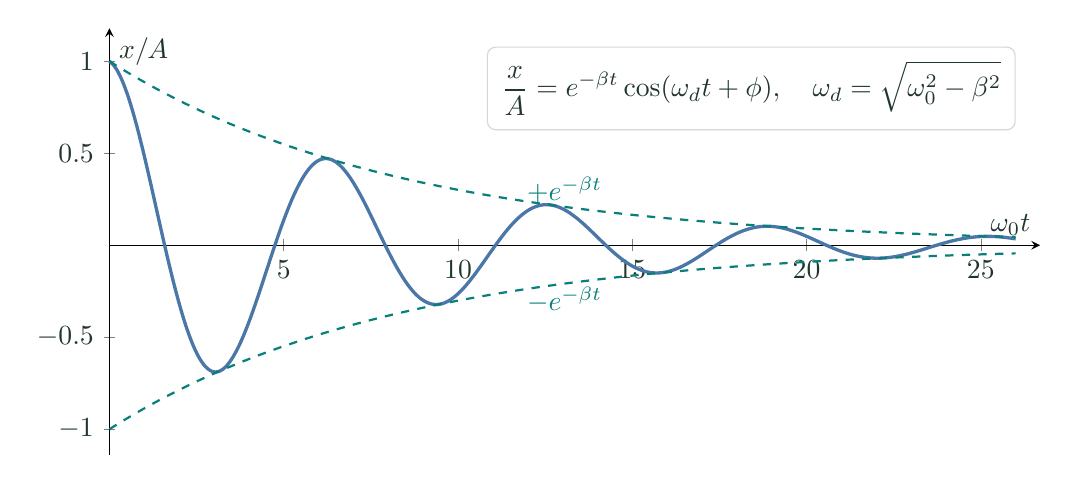
\begin{tikzpicture}[font=\sffamily,text=ink]
\begin{axis}[
  width=13.4cm,height=7cm,
  axis lines=middle,
  xmin=0,xmax=26.7,ymin=-1.14,ymax=1.18,
  xlabel={$\omega_0t$},ylabel={$x/A$},
  ytick={-1,-.5,0,.5,1},
  xtick={0,5,10,15,20,25},
  domain=0:26,samples=520,clip=false
]
  % beta/omega_0 = 0.12, so omega_d/omega_0 = sqrt(1-0.12^2).
  \addplot[blue,very thick]
    {exp(-0.12*x)*cos(deg(sqrt(1-0.12^2)*x))};
  \addplot[teal,thick,dashed,samples=220] {exp(-0.12*x)};
  \addplot[teal,thick,dashed,samples=220] {-exp(-0.12*x)};
  \node[teal,anchor=west] at (axis cs:11.7,.30)
    {$+e^{-\beta t}$};
  \node[teal,anchor=west] at (axis cs:11.7,-.30)
    {$-e^{-\beta t}$};
  \node[draw=ink!20,rounded corners=3pt,fill=white,anchor=north east,
        inner sep=5pt] at (axis cs:26,1.08)
    {$\displaystyle \frac{x}{A}=e^{-\beta t}\cos(\omega_dt+\phi),\quad
      \omega_d=\sqrt{\omega_0^2-\beta^2}$};
\end{axis}
\end{tikzpicture}
\end{document}
